% --- V-JEPA: Motivation and Overview ---
\begin{frame}{From Images to Video: V-JEPA Motivation}
  \begin{itemize}
    \item The visual world is dynamic: understanding actions and events requires temporal structure.
    \item \textbf{V-JEPA} (Video Joint Embedding Predictive Architecture, Meta) extends the JEPA idea to video: predict \emph{representations} of masked spatio-temporal content, not pixels.
    \item Like I-JEPA, it is \textbf{non-generative}: learning targets live in a learned latent space, so the model can ignore unpredictable detail.
    \item Pre-training uses \textbf{unlabeled video}; labeled data is reserved for lightweight adaptation.
  \end{itemize}
\end{frame}

% --- V-JEPA: Latent-space prediction (Meta blog) ---
\begin{frame}{V-JEPA: Learning in Representation Space}
  \begin{columns}[T,onlytextwidth]
    \column{0.42\textwidth}
    \begin{itemize}\itemsep0.35em
      \item Encoder trained by predicting masked spatio-temporal regions in a \textbf{learned latent space}---analogous to I-JEPA comparing abstract image embeddings rather than pixels.
      \item Self-supervised pre-training on diverse video; task labels used only after pre-training.
    \end{itemize}
    \column{0.56\textwidth}
    \centering
    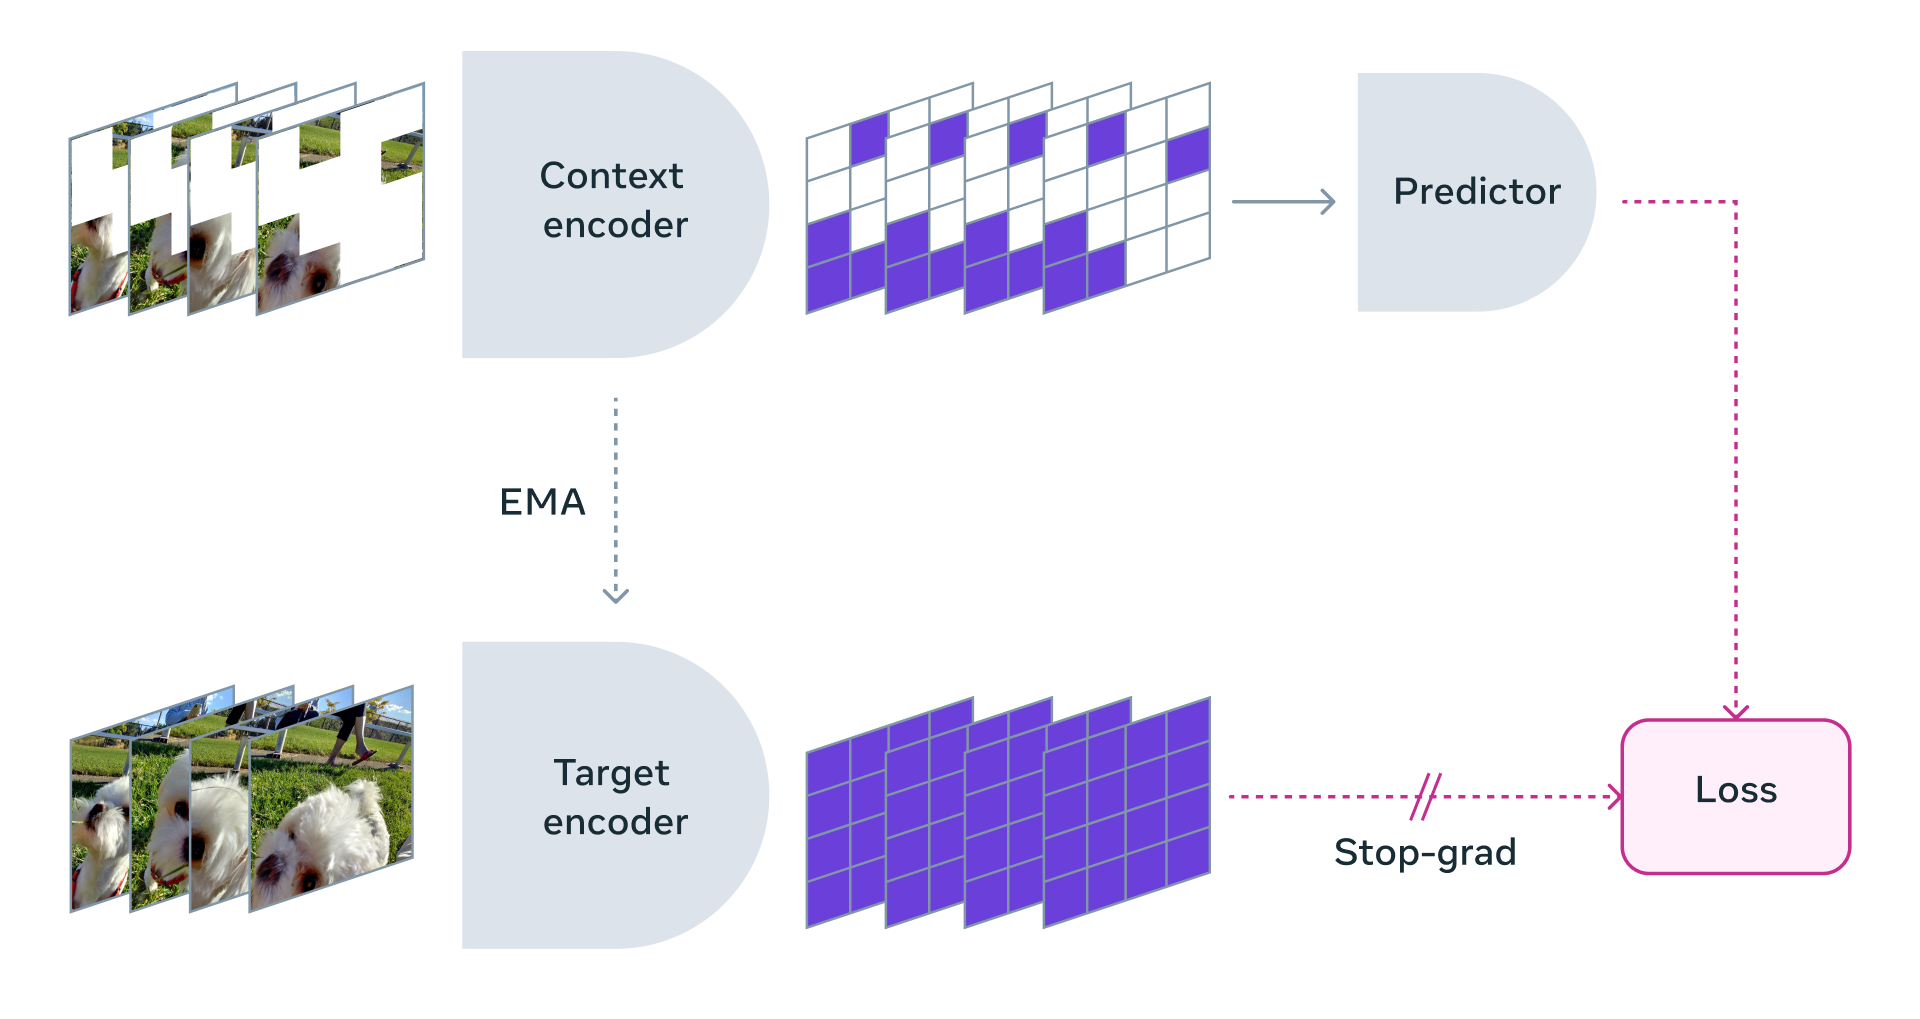
\includegraphics[width=0.9\linewidth, height=0.9\textheight, keepaspectratio]{assets/New-Lecture_JEPA_models/vjepa_encoder_training.png}\\[0.25em]
    {\scriptsize Encoder trained by predicting masked regions in latent space (not pixels). Reference: \href{https://arxiv.org/abs/2404.08471}{V-JEPA paper (Bardes et al., 2024)}.}
  \end{columns}
\end{frame}

% --- V-JEPA: Spatiotemporal masking (Meta blog) ---
\begin{frame}{V-JEPA: Masking in Space \emph{and} Time}
  \centering
  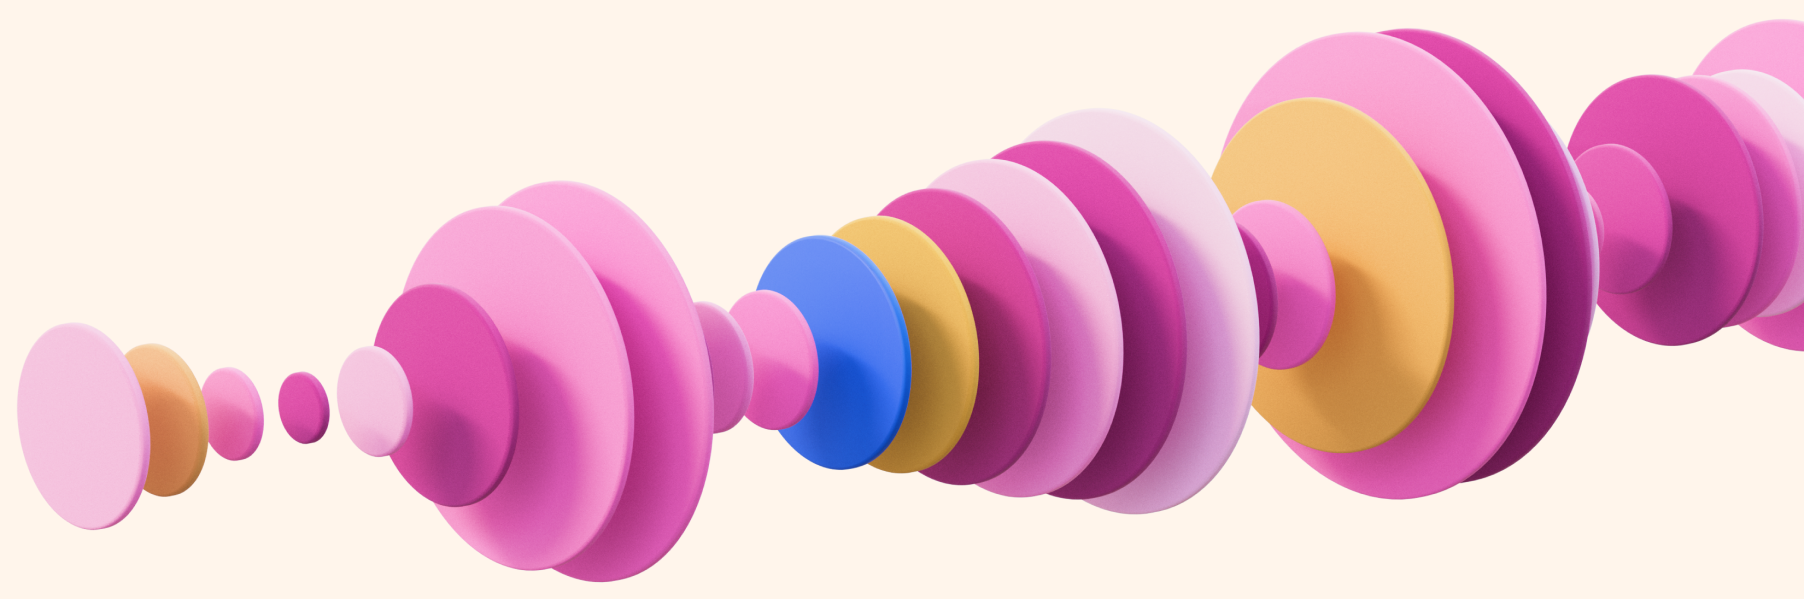
\includegraphics[width=0.8\linewidth, height=0.8\textheight, keepaspectratio]{assets/New-Lecture_JEPA_models/vjepa_blog_spatiotemporal_figure.png}\\[0.25em]
  {\scriptsize Spatio-temporal context and masking. Reference: Meta V-JEPA blog.}
  \begin{itemize}\footnotesize
    \item Masking must be hard enough: \textbf{sparse random patches} make the task too easy---little is learned about dynamics.
    \item If a region is masked only at \textbf{one instant} while adjacent frames stay visible, the model can ``cheat'' from neighboring time steps.
    \item V-JEPA uses masking across \textbf{both space and time} so the model must infer what happens in the scene, not copy texture from nearby frames.
  \end{itemize}
\end{frame}

% --- V-JEPA: Architecture ---
\begin{frame}{V-JEPA: Model Architecture}
  \begin{columns}[T,onlytextwidth]
    \column{0.44\textwidth}
  \begin{itemize}
        \item \textbf{Context path:} encodes visible video patches; \textbf{predictor} maps to the target representation space (JEPA-style).
        \item \textbf{Target path:} encodes masked regions for the training target (with stop-gradient); loss matches predicted and target embeddings.
        \item Same high-level recipe as I-JEPA, extended to \textbf{3D} patch tokens over space and time.
  \end{itemize}
    \column{0.56\textwidth}
      \centering
      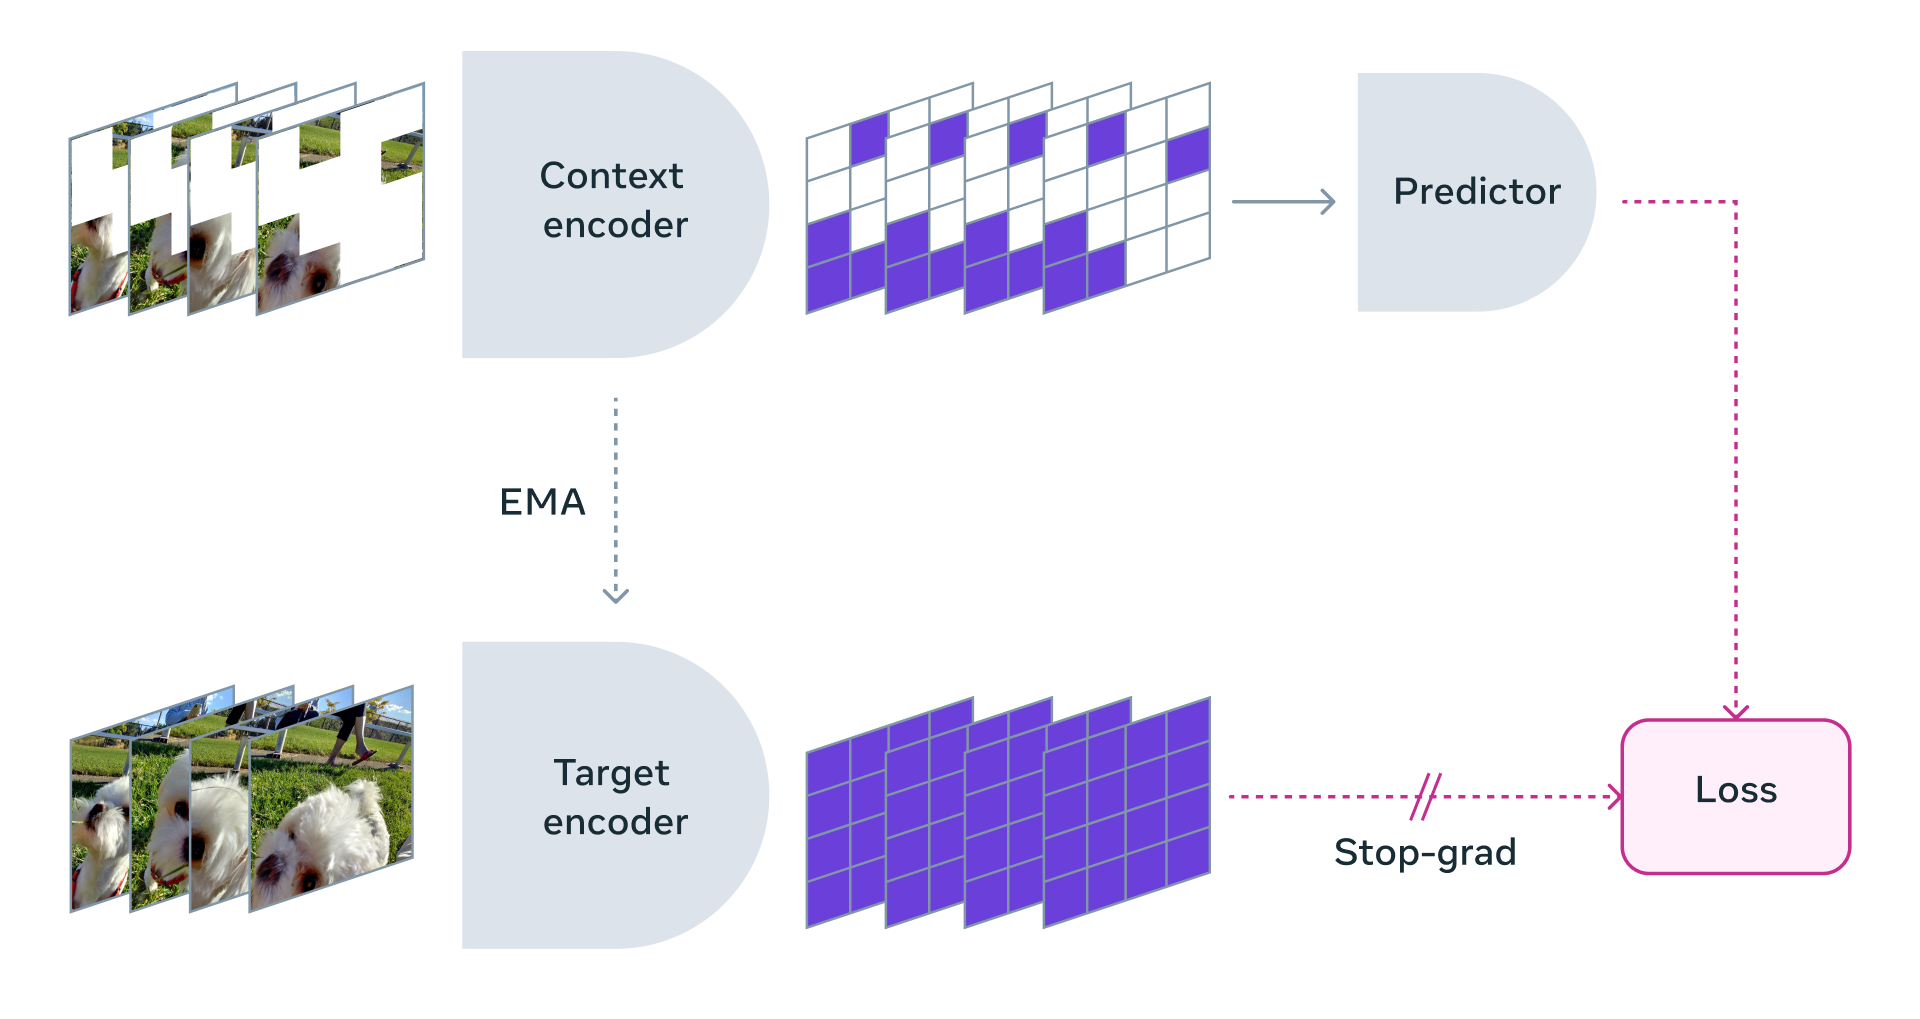
\includegraphics[width=0.95\linewidth, height=0.9\textheight, keepaspectratio]{assets/New-Lecture_JEPA_models/vjepa_encoder_training.png}\\[0.25em]
      {\scriptsize Reference: \href{https://arxiv.org/abs/2404.08471}{V-JEPA paper (Bardes et al., 2024)}.}
  \end{columns}
\end{frame}

% --- V-JEPA: Training Specifics ---
% \begin{frame}{V-JEPA: Training and Implementation}
%   \begin{itemize}
%     \item Built on \textbf{3D ViT}-style backbones and large-scale \textbf{unlabeled} video.
%     \item Augmentations and masking are designed for \textbf{temporal coherence}, motion, and scene continuity---aligned with the space--time masking strategy.
%     \item Predictions in embedding space emphasize \textbf{higher-level} content (e.g., who does what) rather than irrelevant pixel detail (e.g., every leaf on a tree).
%   \end{itemize}
% \end{frame}

% --- V-JEPA: Frozen evaluation (Meta blog) ---
\begin{frame}{V-JEPA: Architecture}
  \begin{columns}[T,onlytextwidth]
    \column{0.42\textwidth}
    \begin{itemize}\itemsep0.35em
      \item After self-supervised pre-training, the \textbf{encoder and predictor are frozen}.
      \item Same frozen backbone can support several tasks (e.g., action classification, fine-grained interaction recognition, activity localization) without full fine-tuning that would specialize the whole network to one benchmark.
  \end{itemize}
    \column{0.56\textwidth}
    \centering
    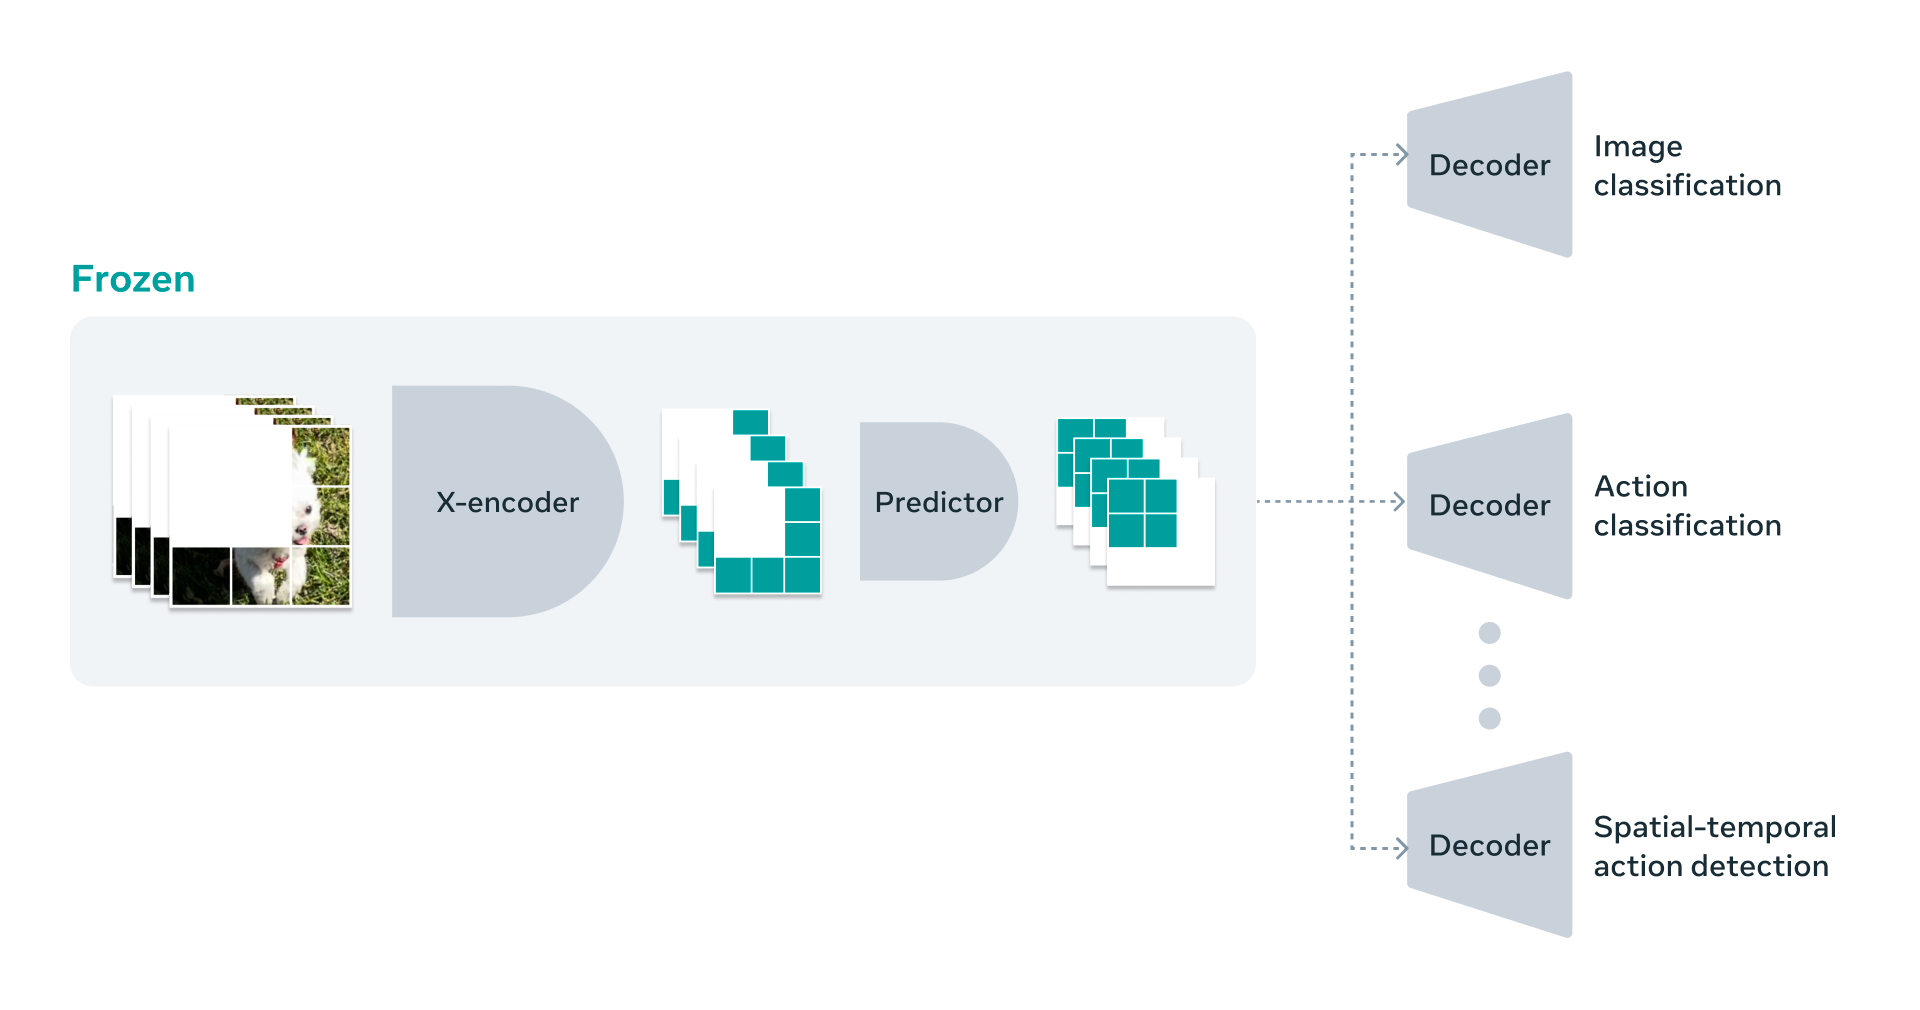
\includegraphics[width=0.95\linewidth, height=0.9\textheight, keepaspectratio]{assets/New-Lecture_JEPA_models/vjepa_downstream_tasks.png}\\[0.25em]
    {\scriptsize Reusing frozen representations for downstream video understanding. Reference: \href{https://arxiv.org/abs/2404.08471}{V-JEPA paper (Bardes et al., 2024)}.}
  \end{columns}
\end{frame}

% --- V-JEPA: Low-shot frozen evaluation (Meta blog) ---
% \begin{frame}{V-JEPA: Results}
%   \begin{columns}[T,onlytextwidth]
%     \column{0.38\textwidth}
%     \begin{itemize}\itemsep0.3em
%       \item \textbf{Frozen evaluation:} probes trained on a fraction of labels (e.g., 5\%, 10\%, 50\% of the training set per class) on Kinetics-400 and Something-Something-v2, with multiple random splits.
%       \item As supervision gets scarcer, the gap between V-JEPA and baselines tends to \textbf{grow}---strong sample efficiency for the frozen encoder.
%     \end{itemize}
%     \column{0.6\textwidth}
%     \centering
%     \includegraphics[width=0.8\linewidth, height=0.8\textheight, keepaspectratio]{assets/New-Lecture_JEPA_models/
%     vjepa_blog_eval_chart.png}\\[0.25em]
%     {\scriptsize Low-shot frozen evaluation on K400 / SSv2. Reference: Meta V-JEPA blog.}
%   \end{columns}
% \end{frame}

% --- V-JEPA: Capabilities and Evaluation ---
\begin{frame}{V-JEPA: Results, and Limitations}
  \begin{itemize}
    \item Strong on \textbf{frozen} benchmarks spanning image/video classification, action recognition, and spatio-temporal action detection relative to prior video representation learning.
    \item Particularly strong on \textbf{fine-grained} interaction understanding over short clips (e.g., distinguishing put-down vs.\ pick-up vs.\ pretend actions).
    \item Reported limitations include \textbf{short clip} focus (on the order of seconds); \textbf{audio} and \textbf{long-horizon} prediction/planning highlighted as future directions.
  \end{itemize}
  \centering
  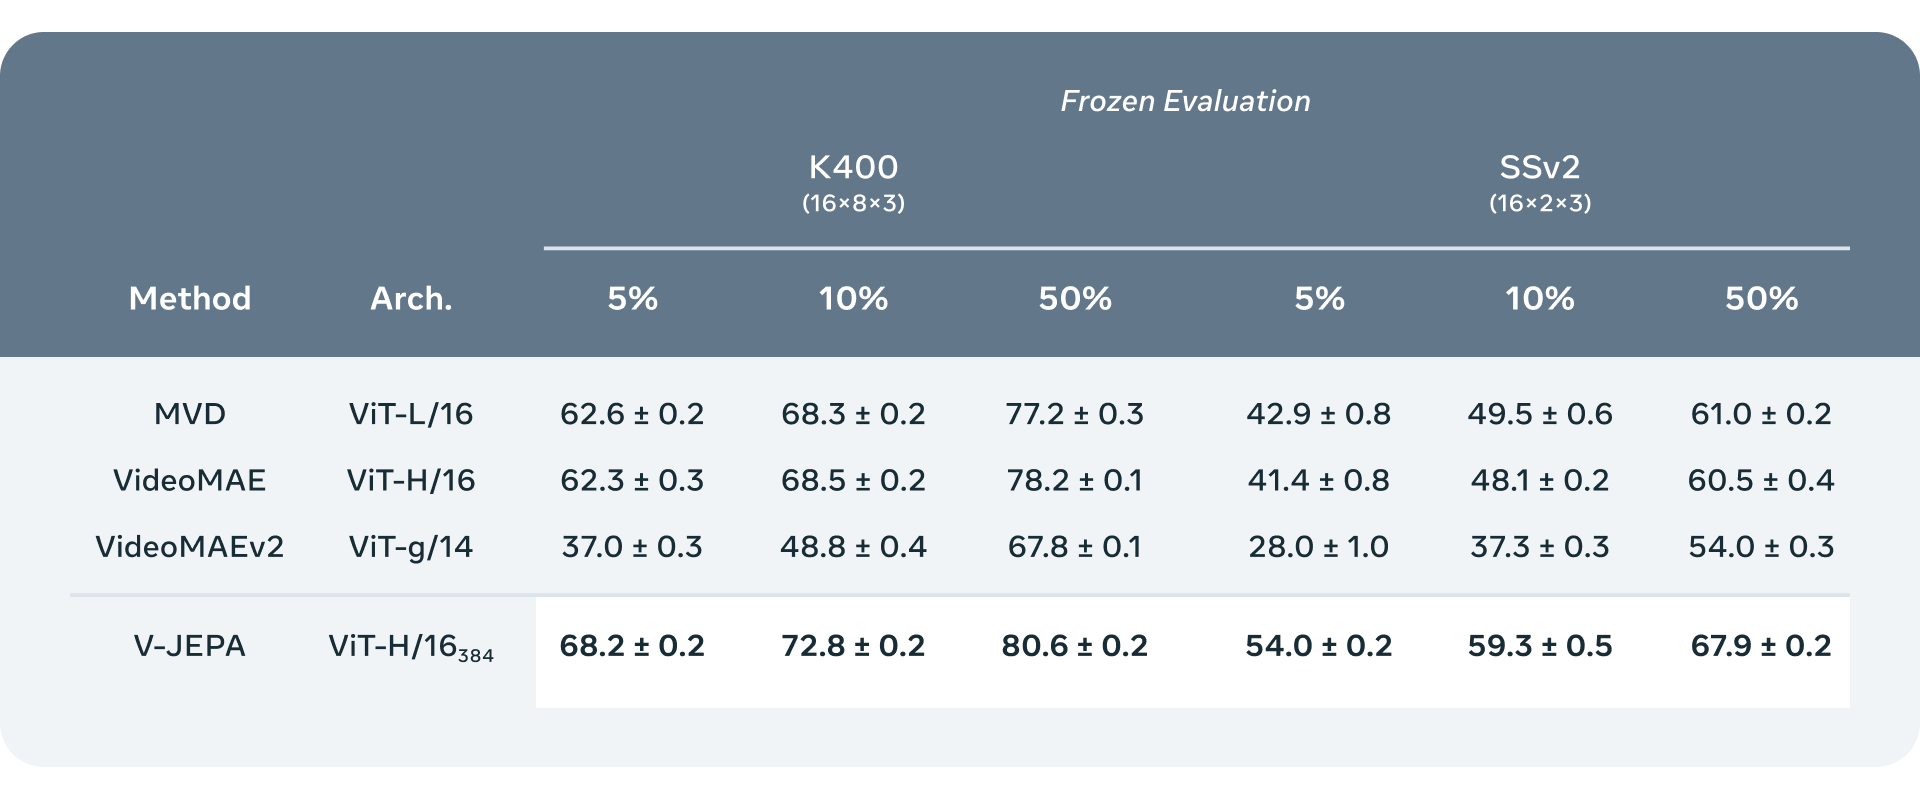
\includegraphics[width=0.8\linewidth, height=0.5\textheight, keepaspectratio]{assets/New-Lecture_JEPA_models/vjepa_blog_eval_chart.png}\\[0.25em]
  {\scriptsize Low-shot frozen evaluation: Comparing V-JEPA to other video models in frozen evaluation on Kinetics-400 and Something-Something-v2 (Meta V-JEPA blog; \href{https://arxiv.org/abs/2404.08471}{V-JEPA, Bardes et al.}).}
\end{frame}
